\subsection{PMT surface coating}

The PMTs used in the LTCC are Photonis XP4500Bs \cite{Photonis:2007ta}.
Their borosilicate windows can be used to detect wavelengths as low as approximately
300 nm. This is the most limiting factor of enhanced quantum efficiency (QE) in the UV region, where most of the Cherenkov
light is emitted (see eq.~\ref{eq:cerenkov}), given that the $C_4F_{10}$ gas is transparent down to
wavelengths of 180 nm, and the mirrors and WC reflectivity is non-zero
even for wavelengths below 200 nm.
While quartz windows maximize the UV-sensitivity of the PMT, they are difficult and expensive to produce.
A wavelength shifter (WLS) deposited on the face of a borosilicate or UV glass
PMT provides an effective alternative to boost the efficiency of a Cherenkov
detector by converting UV photons with a wavelength below 300 nm into two
isotropically emitted photons with longer wavelengths.

The projected QE gained by a deposition of p-terphenyl (PT) on the XP4500Bs
PMT \cite{Koczon:1457653} is shown in \F{pmtQuantumEfficiencyGainAndExample}.
The gain at shorter wavelengths near 200 nm, where most of the Cherenkov light
detectable by the LTCC optics is concentrated, is more than a factor of 3.


\begin{figure}
	\centering
	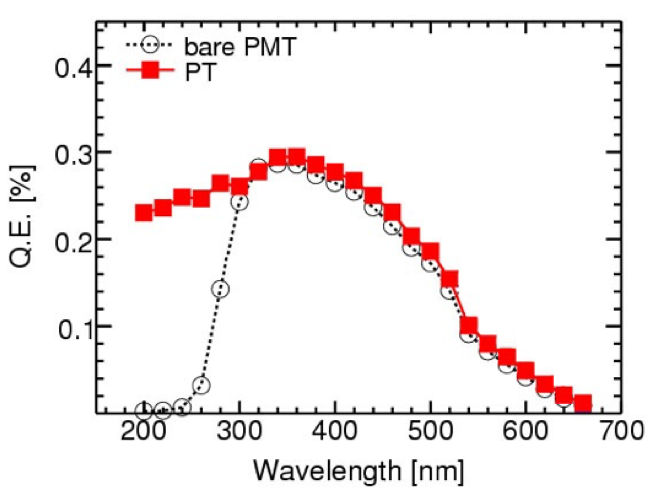
\includegraphics[width=0.99\columnwidth, height=0.65\columnwidth]{img/pmtQuantumEfficiencyGain.png}
%	\includegraphics[width=0.95\columnwidth, height=0.55\columnwidth]{img/ptExample.png}
	\caption{The typical QE for a Photonis XP4500B PMT (solid black line), compared to the projected QE after application
			 of a PT wave-length shifter at four different material loads (dashed lines), as a function of wavelength}
	\label{fig:pmtQuantumEfficiencyGainAndExample}
\end{figure}

Several tests were performed in collaboration with the Temple University Physics Department using the equipment schematics
shown in \F{pmtTestingSetupAndptQEResults} (top). The setup used a monochromator with a precision of 0.35 nm and two PMTs
(one for the measurement, one for the   reference calibration). The PMTs were switched to confirm the stability of the results.
Each PMT was measured while coated and then again after the coating had been removed using acetone and isopropanol.
The observed photon rate was read out by a scaler.

\begin{figure}
	\centering
	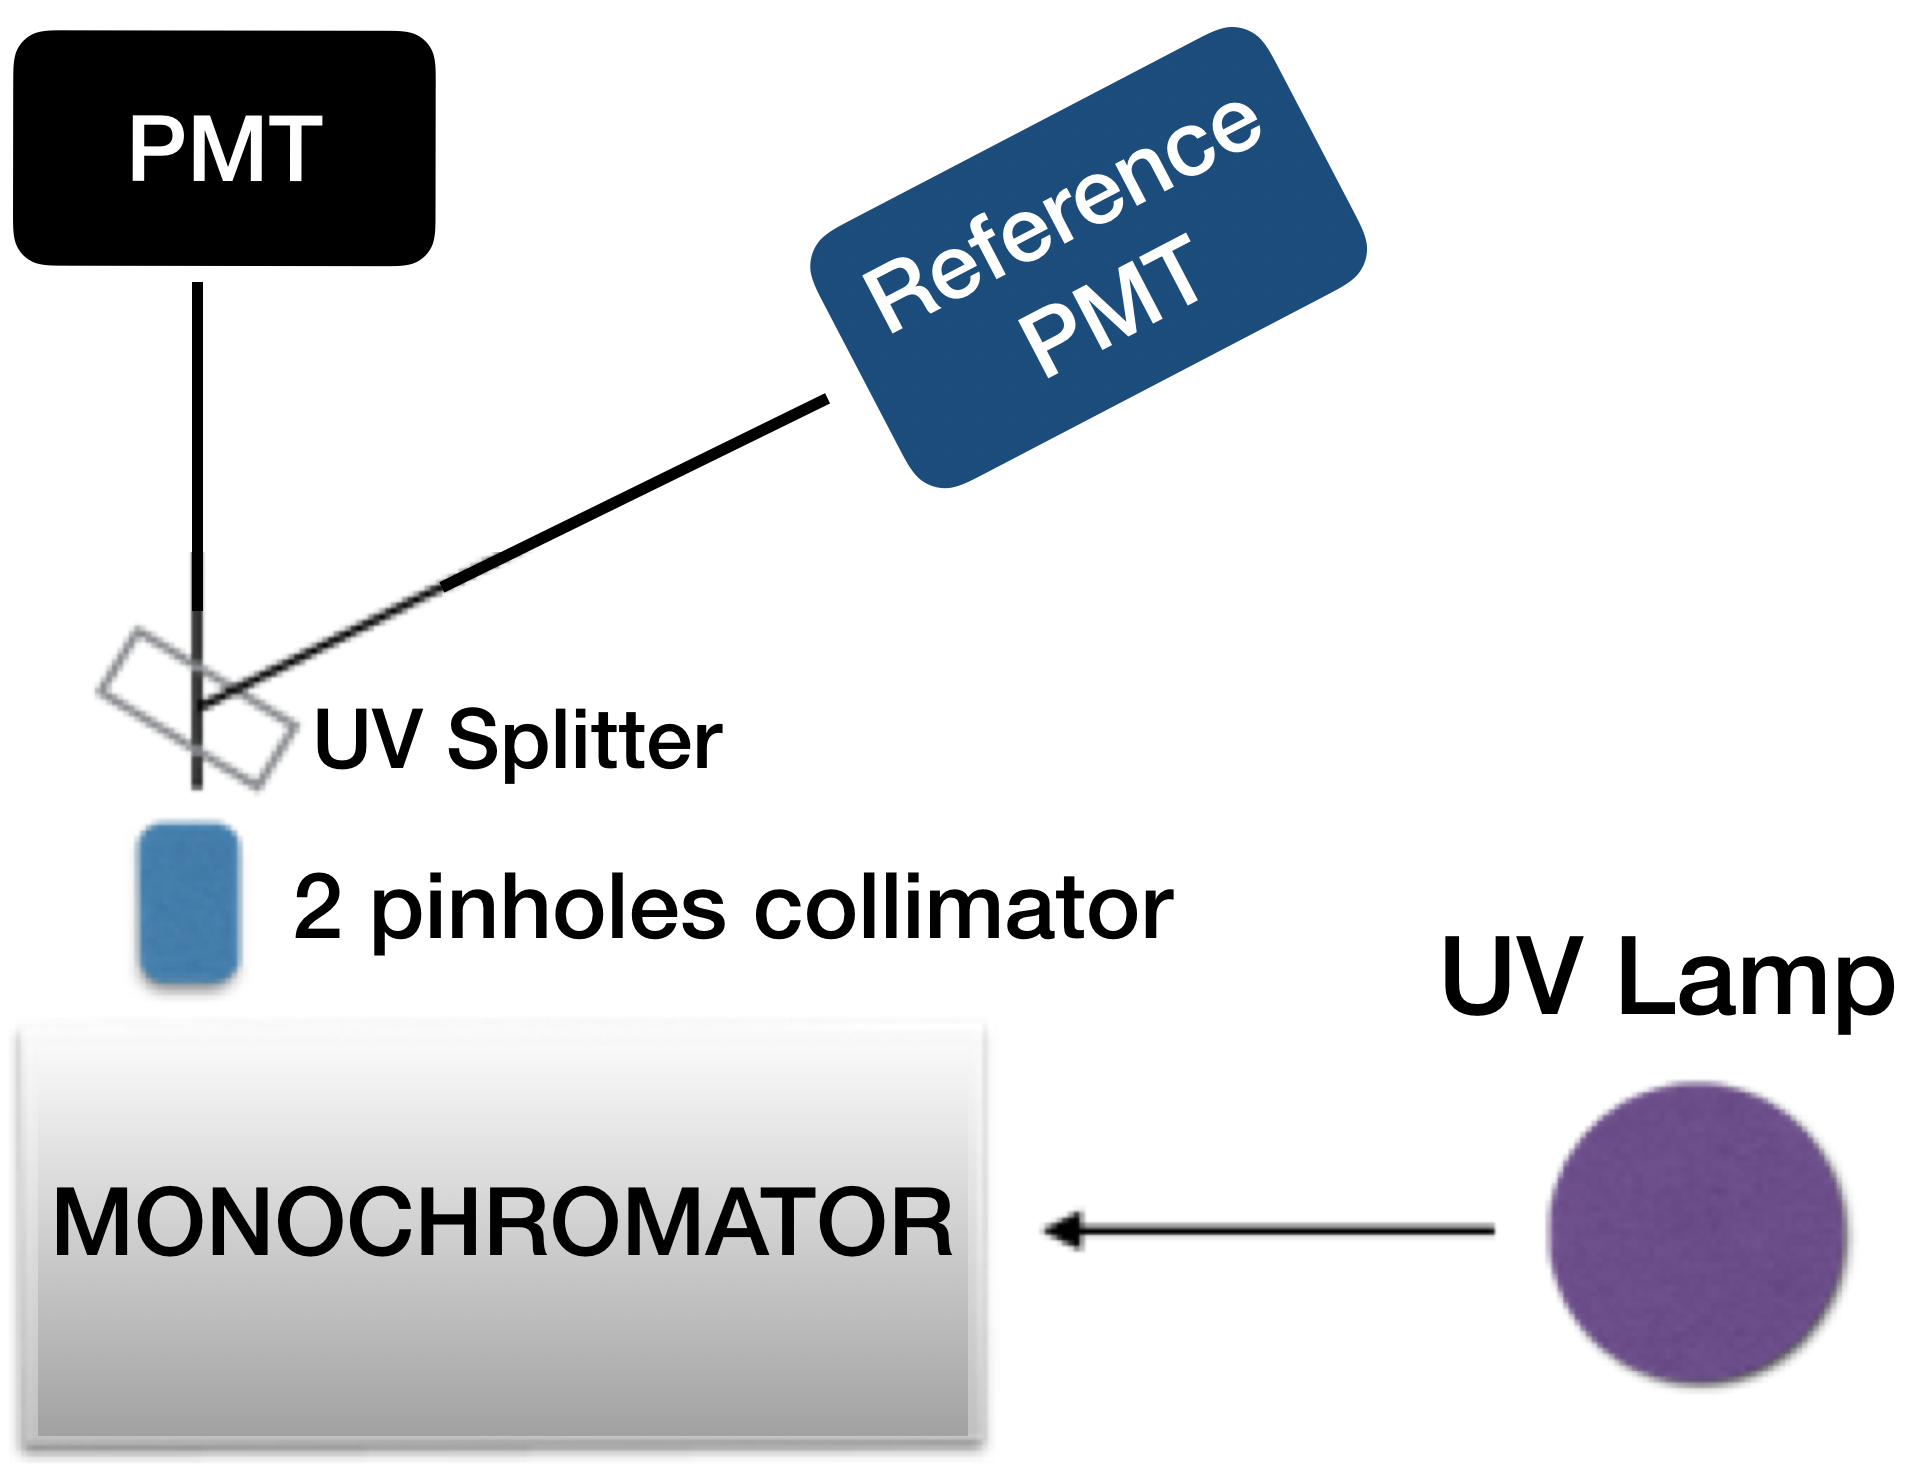
\includegraphics[width=0.95\columnwidth, height=0.65\columnwidth]{img/pmtTestingSetup.png}
	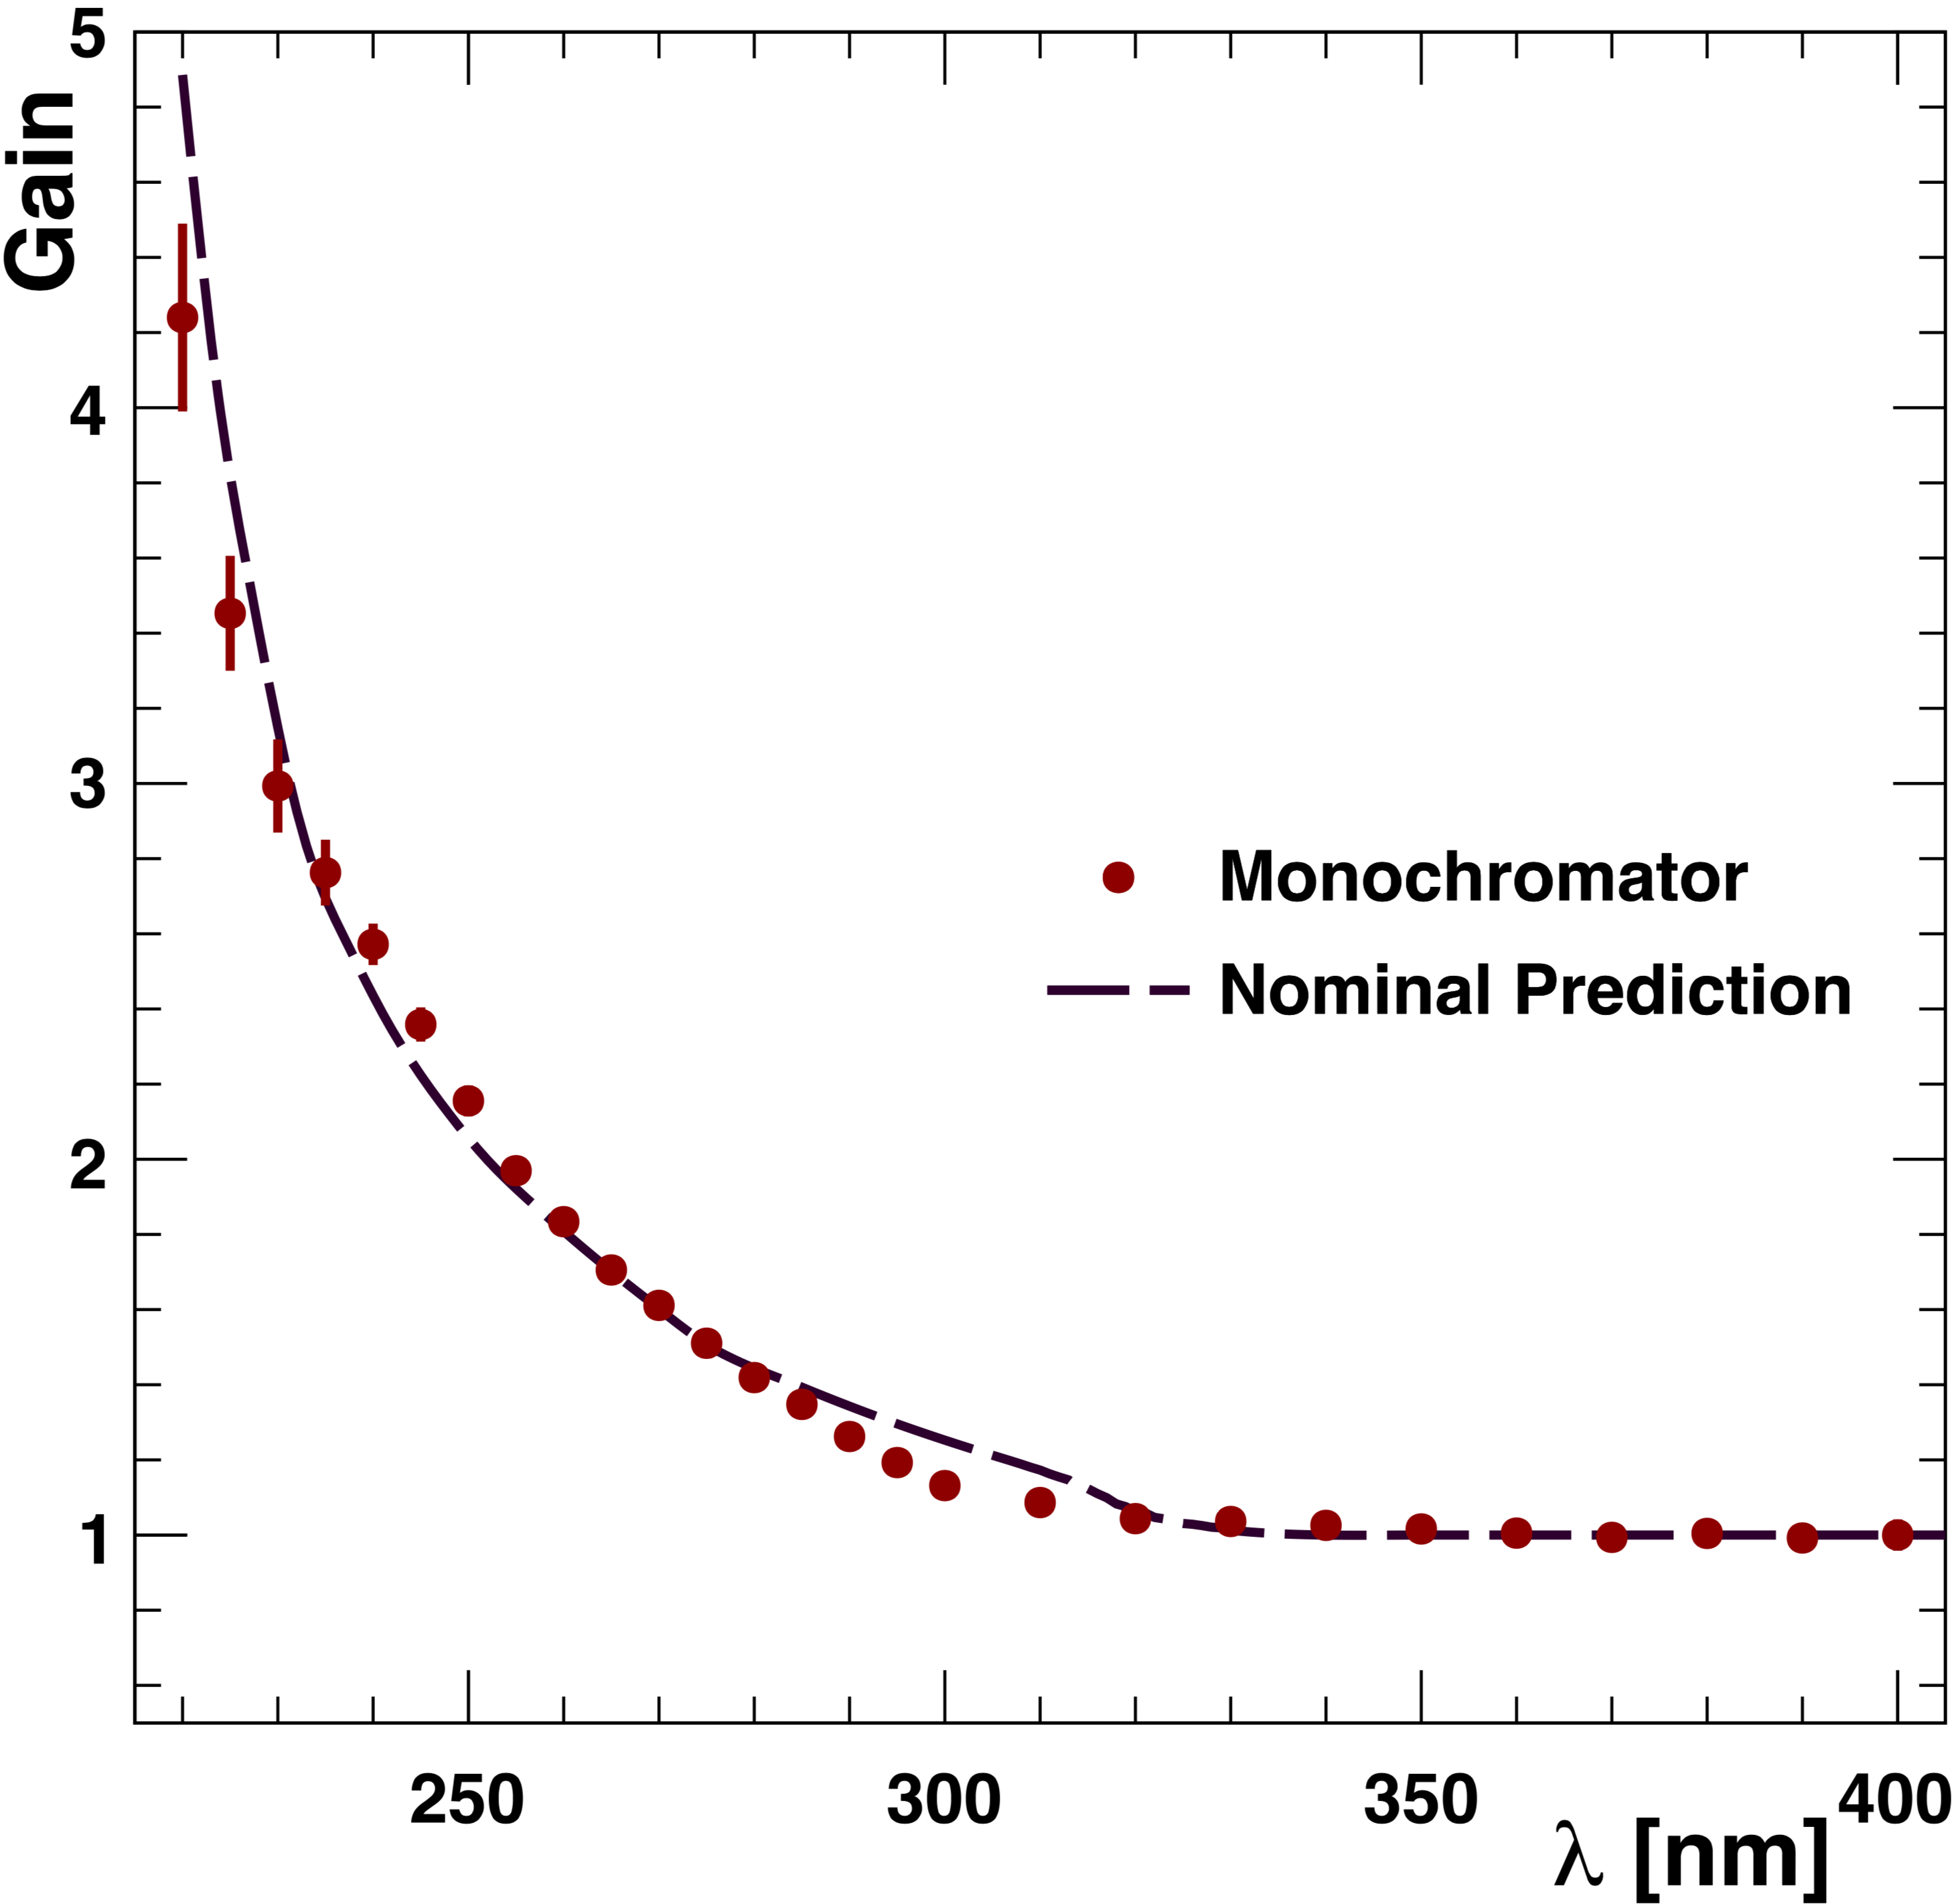
\includegraphics[width=0.99\columnwidth, height=0.65\columnwidth]{img/ptQEResults.png}
	\caption{Top: Monochromator setup used for the gain measurement. Bottom: Results from the monochromator measurements (red circles), compared to the
				nominal prediction for a PT material load of $110\,\mu$ g/cm$^2$ (dashed line).}
	\label{fig:pmtTestingSetupAndptQEResults}
\end{figure}

The results from 2 different PMTs each at 2 different positions were found to be
consistent. \F{pmtTestingSetupAndptQEResults} (bottom) shows the average measured gain from these four
measurements. The observed gain was found to be consistent with the nominal
prediction for a perfectly saturated coating.

Based on these results, 200 PMTs were treated \cite{Joosten:2016lcl} with an optimal material load of 110 $\mu$g/cm$^2$,
corresponding to a PT thickness of 894 nm. This corresponded to an overall
increase of the PMT response to Cherenkov light of about 40\%. The 110 $\mu$ g/cm$^2$ (894 nm) of PT provides an
almost transparent coating to the visible light spectrum.





